% Sample apostrophy's to remove team's 

\title{Lessons Learned from Grappling with a 2.5 Year Participant Observation Study: Emergence of a Constructivist Grounded Theory Researcher: }

\author{
\IEEEauthorblockN{ Todd Sedano }
\IEEEauthorblockA{Pivotal \\
  3495 Deer Creak Road \\
  Palo Alto, CA \\
  Email: professor@gmail.com}
}
% make the title area
\maketitle

\section{Abstract}
 \textit{Context:} Conducting a Grounded Theory study is rigorous, demanding, and challenging. Misperceptions exist within the software engineering community \cite{StolGroundedTheory}.

\textit{Objective:} The purpose of this paper is to describe one extended participant observation Grounded Theory study for aiding new empirical researchers wanting to run similar research studies.

\textit{Method:} Following Constructivist Grounded Theory, we conducted a \durationOfResearchStudy{} participant-observation of \numberOfObservedProjects{} software development projects at Pivotal, a software development organization, interviewed \numberOfInterviews{} software engineers, interaction designers, and product managers, and analyzed one year of retrospection topics. We iterated between analysis and theoretical sampling until achieving theoretical saturation.

\textit{Results:}  This paper describes the mis-steps, challenges, and unique insights that occurred while conducting a Grounded Theory study.

\textit{Limitations:} While the process and results are highly relevant to the researcher, the outcomes might not apply to other researchers.

\textit{Conclusion:} Conducting my own Grounded Theory research study, attending Glaser's Seminar, and reading and re-reading Charmaz's and Glaser's books helped the researcher overcoming misperceptions about Grounded Theory research.
\section{Introduction}

\participantQuote{Grounded Theory is such a simple method, yet so easily and often misapplied \cite{StolGroundedTheory}. It is easy to describe but hard to understand. My Grounded Theory study appears typical: confusion followed by insight. A researcher starts a Grounded Theory study open to see where the research leads. Once unleashed, the method seems to have a mind of its own as it guides the researcher towards research treasure through uncharted territory. I've been teaching and performing Extreme Programming for over 11 years, yet the method delighted me by finding precious insights}  \textemdash Todd Sedano \footnote{Interviewing oneself is an acceptable practice for participant observation in Grounded Theory even if it may seem like cheating}. 

For the past 2.5 years, I have been conducting a full-time participant observation Grounded Theory study. Lengthy participant observation studies are unusual in software engineering and in computer science more generally. This paper describes my experiences in order to help future researchers considering a similar trajectory. 

My first introduction to Grounded Theory came while reading Bren\'{e} Brown's \underline{Daring Greatly} \cite{BreneBrownDaringGreatly} in March 2013. Brown spends a significant portion of her book detailing her journey in applying Grounded Theory to her psychological research about processing shame. Given my strengths with interpersonal communication, the technique appealed to me. 

While attending ICSE in San Francisco in May 2013, I participated in the first International Workshop on Conducting Empirical Studies in Industry (CESI 2013). I pestered researchers about how they used Grounded Theory in their research. (Thanks to Irit Hadar and Christopher Bull for answering all of my questions.) After the workshop, during the main conference, I sought out each Grounded Theory presentation to learn more about how the community used the method.

The structure of the paper follows the stages of a Grounded Theory study,  Section \ref{GettingStarted} \quotes{Getting started,} Section \ref{Analysis} \quotes{Analysis,} and Section \ref{TheoryConstruction} \quotes{Theory Construction,} and Section \ref{TheoreticalSaturation} \quotes{Theoretical Saturation}.
\section{Getting Started}
\label{GettingStarted}

Following Glaser's advice of \quotes{just do it} \cite{GlaserIssues}, I learned the intricacies of Grounded Theory while conducting my first Grounded Theory study. At each stage of the research, I read the next few chapters to understand what I would be doing next. 

This section examines early important decisions such as which varient to use, selecting a site, and gathering rich data.
\subsection{Selecting a Method Variant}
Given the philosophical differences between the three variants of Grounded Theory, understand why you are selecting that variant. Initially, I chose Constructivist Grounded Theory simply because it was the latest, a fine justification for selecting software libraries, but as I later discovered, not the best reason for selecting a sociological research method. 

I continue to use Constructivist Grounded Theory because it allows for the recording and transcription of interviews, enables literature review when appropriate in the research process, and builds upon decades of Grounded Theory research and experience. The philosophical stance of constructivism (as opposed to positivism) acknowledges the researcher's and participants' contributions to the construction of concepts. Positivistism acknowledges that knowledge from observable facts whereas constructivism posits that knowledge situated in a human context which may be more useful in understanding social interactions. For software engineering research, Constructivist Grounded Theory seems aptly suited since software development is a socio-technical endeavor.

With transcriptions and line-by-line coding, Constructivist Grounded Theory generates a lot of data. Even still, I prefer the slower more intimate coding of Constructivist Grounded Theory.

\textit{Recommendation:} If you want to just get started, begin with Stol's comparison of the three variants \cite{StolGroundedTheory}, read a few software engineering research papers such as \cite{SedanoSustainableSoftware, SedanoSoftwareDevelopmentWaste}, and then read Charmaz's book \cite{Charmaz}. If you want more depth about each variant, read Evan's article \cite{Evans2013novice}. Realize that Evan includes Glaser's pontificating criticisms of Constructivist Grounded Theory \cite{GlaserConstructivistGroundedTheory}, but excludes Bryant's rebuttal \cite{Bryant2007}. 

My primary text was Charmaz \cite{Charmaz}, which I supplemented with Glaser's books \cite{GlaserDiscovery, GlaserTheoreticalSensitivity, GlaserIssues} to build a deeper understanding of the method and the historical context of Constructivist Grounded Theory. Charmaz's textbook is approachable. Glaser tends to jargonize.

\textit{Lesson Learned:} I initially purchased and read Glaser's books in the wrong sequence. His works are additive and build on each other.

\textit{Recommendation:} If you select Constructivist Grounded Theory, start with Charmaz' book \cite{Charmaz}. Read Glaser's books in sequence, about a topic, to better understand the theoretical underpinnings of Grounded Theory. 

\subsection{Selecting a Research Site}
We selected Pivotal because: 1) it is successful; 2) it is interesting in its continued use and evolution of extreme programming; 3) it is accessible and cooperative with research. Both Classic and Constructivist Grounded Theory advocate picking an interesting site to see \quotes{What's going on here?} 

Pivotal Labs is a division of Pivotal\textemdash a large American software company (with 17 offices around the world). Pivotal Labs provides teams of agile developers, product managers, and interaction designers to other firms. Its mission is not only to deliver highly-crafted software products but also to help transform clients' engineering cultures. To change the client's development process, Pivotal combines the client's software engineers with Pivotal's engineers at a Pivotal office where they can experience Extreme Programming \cite{BeckExtremeProgramming2004} in an environment conducive to agile development. Pivotal Labs has followed Extreme Programming \cite{BeckExtremeProgramming2004} since the late 1990's. 

\textit{Lessons learned:} We found selecting a consultancy to be helpful as they were open to us researching the way they work provided we did not reveal information about the client. The client owns the code, not the way of working. Revealing insights about Pivotal Labs aligned with its business goals. A consultancy provides exposure to many different projects, both greenfield and brownfield. Client-pivotal dynamics revealed the tension of adopting agile software development. A consultancy's focus on billing 40 hours a week required research activities (e.g. data collection, data analysis, and attending conferences) to be done on personal time.

\textit{Recommendation:} Since Grounded Theory starts with the question, \quotes{what is going on here?} start with an organization that excels at what you hope to research.
\subsection{Gathering Rich Data}
The research study started with data from two sources: 1) interviews with Pivotal employees and 2) participant observation. When starting data collection, I had no notion of the number of interviews or amount of participant observation that I would conduct. 

\textbf{Interviews:} The interviewees consisted of interaction designers, product managers, and software engineers who had experience with Pivotal's software development process from five different Pivotal offices. 

Interview candidates were selected opportunistically. If a Product Manager from the New York office visited the Palo Alto office, I would attempt to schedule an interview that day. When I visited the Los Angeles area for a vacation, I scheduled interviews at the Santa Monica office. 

\textit{Lesson Learned:} With opportunistic interviewing, it is easy to build a backlog of interviews to transcribe and code. 

\textit{Recommendation:} Code and begin constant comparison promptly.

\textit{Lesson learned:} Opportunistic interviewing sometimes built a backlog of interviews for me to transcribe, code, and analyze with constant comparison. 

\textit{Recommendation:} Begin coding as soon as possible. Prioritize coding interviews over conducting another opportunistic interview. 

I relied on \quotes{intensive interviews,} which are \quotes{open-ended yet directed, shaped yet emergent, and paced yet unrestricted} \cite{Charmaz}. Open-ended questions were used to enter into the participant's personal perspective within the context of the research question. The interviewer attempts to abandon assumptions to better understand and explore the interviewee's perspective. Charmaz \cite{Charmaz} contrasts intensive interviews with informational interviews (collecting facts), and investigative interviews (exposing hidden intentions, practices or policies).

\textit{Lesson Learned:} Creating an interview guide helped me generate open-ended questions. Transcribing and coding my interviews enabled me to hear when I asked leading questions.

\textit{Recommendation:} Create an interview guide and use it only three times. Constant comparison needs to direct questions in the interview.

The initial interviews were open-ended explorations starting with the question, \quotes{Please draw on this sheet of paper your view of Pivotal's software development process.} My goal was not to force initial topics and understand the perspective of the interviewee. Figure \ref{2015_08_12_simple} shows a simple drawing and Figure \ref{2015_08_12_detailed} shows a detailed drawing. 

\begin{figure}[htbp]
\centering
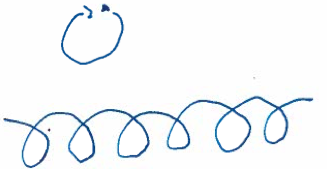
\includegraphics[width=\oneColumnWidth{}]{drawings/interview8.png}
\caption{Interview 8: Simple drawing of Pivotal's software development process}
\label{2015_08_12_simple}
\end{figure}

\begin{figure}[htbp]
\centering
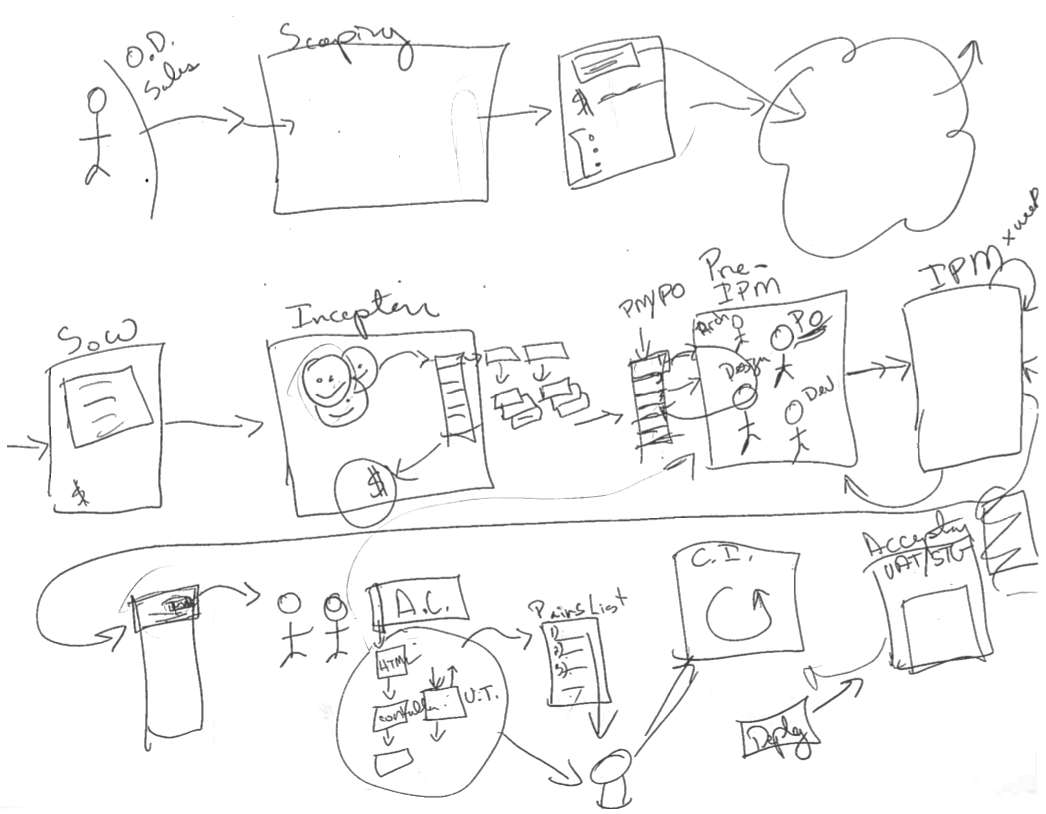
\includegraphics[width=\oneColumnWidth{}]{drawings/2015_08_12_anchor.png}
\caption{Interview 6: Detailed drawing of Pivotal's Software Development process}
\label{2015_08_12_detailed}
\end{figure}

When analysis shifted interviewing onto new topics, I would start with a new drawing question. Asking participants, \quotes{please draw your feelings about the code} often resulted in conversations about code ownership. Figure \ref{Interview31} shows an example. 

\begin{figure}[htbp]
\centering
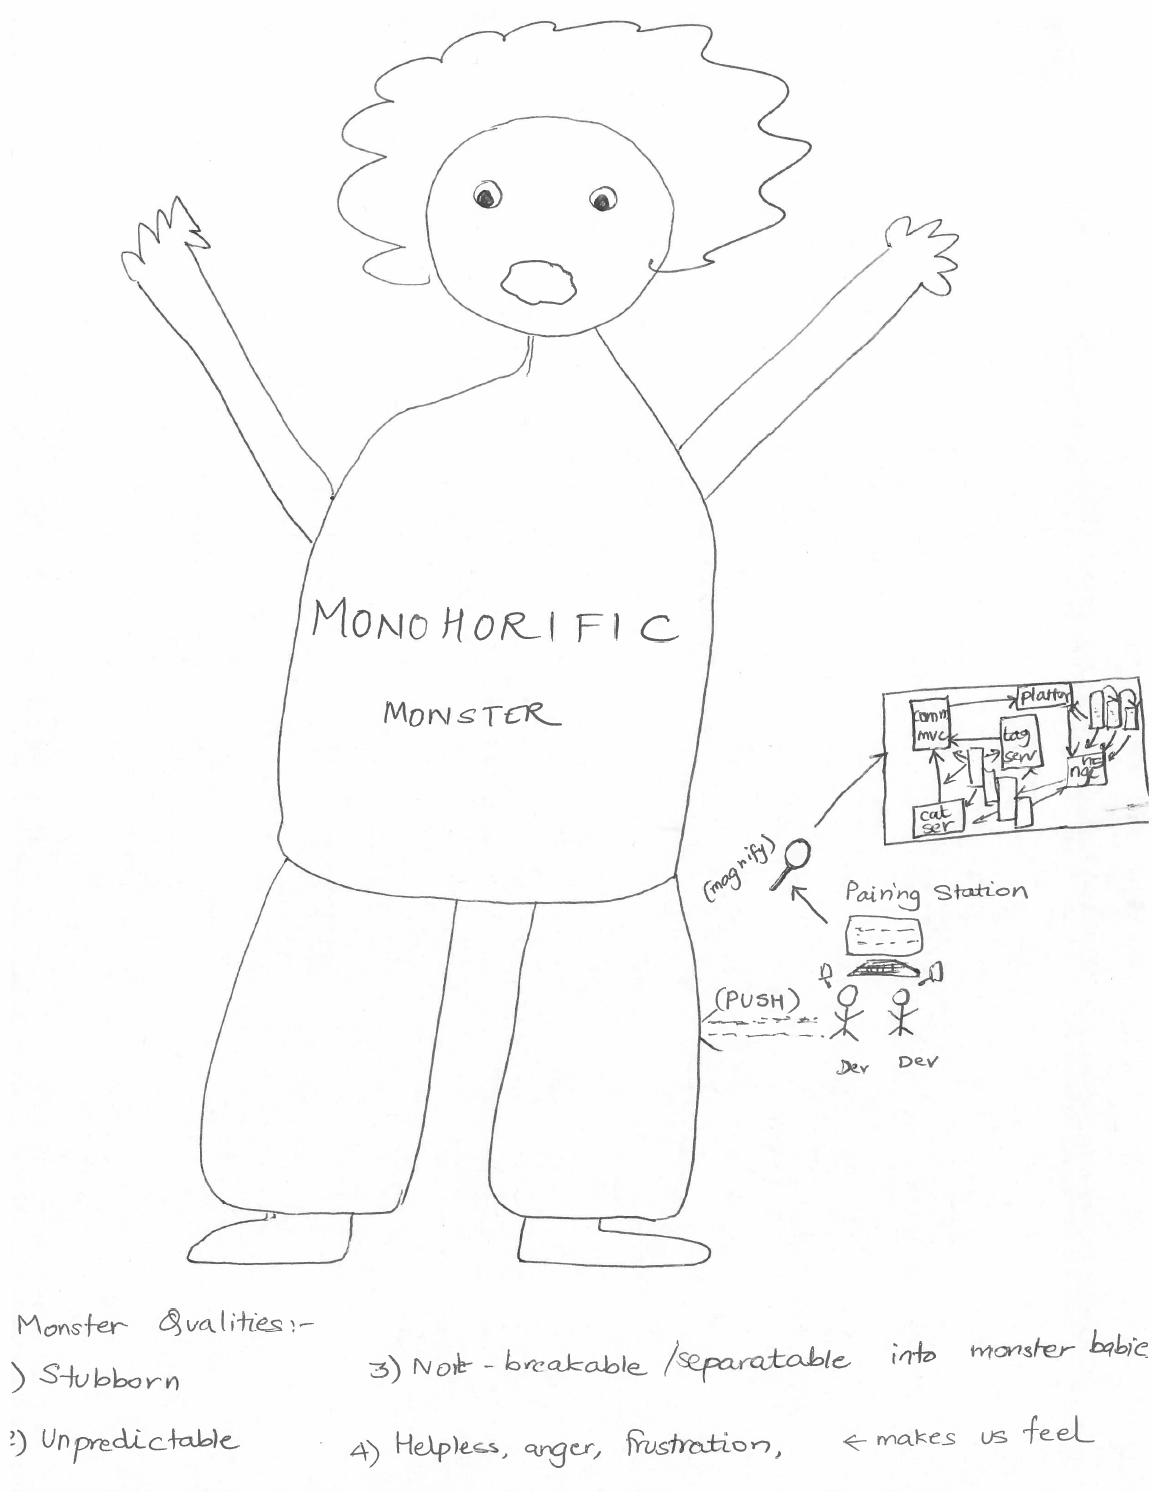
\includegraphics[width=\oneColumnWidth{}]{drawings/2016_09_26.png}
\caption{Interview 31: Software Engineer's drawing for \quotes{How you feel or how you think about the code'}}
\label{Interview31}
\end{figure}

\textit{Lesson Learned:} Asking participants to draw provided a natural starting place for follow-up questions without forcing topics or perspectives.

\textit{Recommendation:} Start interviewing with a \quotes{Sedano} drawing question.

\textbf{Participant Observation:} While working as an engineer, I participated on \numberOfObservedProjects{} sequential projects lasting \durationOfResearchStudyPlural{}. I collected field notes that describe individual and collective actions, capture what participants found interesting or problematic, and include anecdotes and observations. For details about each project see our paper on software development waste \cite{SedanoSoftwareDevelopmentWaste}.

Here is a portion of a field note: 
\participantQuote{Monday was the first time we started getting data from the client's servers. We've been implementing for several months without knowing whether our system would work with real backend systems. In order to make progress, we created mocks for each of the client's systems based upon documentation. Now we need to modify our code base to match the reality of the systems' implementation.}

\textit{Lesson Learned:} Collecting and analyzing field notes from participant observation is not easy. At the beginning of her research, Charmaz pictured a research experience where she would observe her research participants during the day and disappear into the coffee room to take detailed notes and write up her experience \cite{Charmaz}. She discovered that this is challenging in practice, as it can be difficult to disappear while observing activities. When the participant activity is intensive, such as the case with pair-programming, recording observations is tricky. I relied on small notes on post-it notes (which were culturally acceptable compared to typing on a laptop) and detailed observations after work.

\textit{Recommendation:} Use post it notes for capturing insights during pair programming. Explain what you are doing to your pair. For example, \quotes{I want to reflect on what you said} or \quotes{what you said was really insightful} makes the participant feel valued. Record verbal notes on the drive home; some phones will convert spoken words into text.
\section{ Analysis (Coding and Constant Comparison) }
\label{Analysis}
Data analysis began by iteratively collecting and analyzing interview transcripts and participant observations. I used line-by-line coding \cite{Charmaz} to identify nuanced interactions in the data and avoid jumping to conclusions. Whenever insight occurred, I would write it down as a memo.

My advisor reviewed the initial codes while reading the transcripts and listening to the audio recordings.  We discussed the codes and the coding process during weekly research collaboration meetings. To avoid missing insights from these discussions \cite{GlaserTheoreticalSensitivity}, we often recorded and transcribed the discussion into Grounded Theory memos. As data was collected and coded, I stored initial codes in a spreadsheet and I used constant comparison to generate focused codes.

\textit{Lesson Learned:} In retrospection, I have a personal tendency to continue too long with initial coding. When opening a transcript, I enter a comforting, familiar routine. 

\textit{Recommendation:} Use constant comparison to drive research forward.

\subsection{Understanding Constant Comparison}
I attended Glaser's Grounded Theory Seminar in Mill Valley, CA hoping to better understand constant comparison. Glaser structures the workshop to help aid the attending researchers to move from their current phase to the next phase of the Grounded Theory process, not transition them to the final step. Glaser intentionally challenges a participant's point of view. From his perspective, an attendee having an emotional breakdown is a sign of a successful workshop.

Here's a personal memo from my experience, \participantQuote{Before my turn, he tore into a participant for bringing pre-conceived notions into the research. At the last moment, I changed my question for him. I regret that I panicked.  I'm kicking myself for not being true to my original question.  I am very glad to have a deeper understanding of Glaser's approach (since it is so hard to reverse engineer it from his books.) I feel like a failure, even though I am very happy with the work that I have done.}

The workshop helped me understand the fundamental terms used in Grounded Theory. At the time, I was reading through three of Glaser's books \cite{GlaserDiscovery, GlaserIssues, GlaserTheoreticalSensitivity} and I was struggling to understand constant comparison and the conversion of codes into categories. These books do not clearly define the terms; distinguish the differences between the terms; nor provide clear examples illustrating the concepts. Listening to Glaser discuss the concepts helped me solidify what he meant by each term. Later, I discovered that another Glaser book \cite{GlaserBasics} does define the terms in response to Strauss and Corbin's book \cite{Strauss1988Basics}.

\textit{Lesson Learned:} I needed to buy four of Glaser's books to properly understand his method.

Glaser's seminal book assumes the reader is a sociologist. The terms can be confusing. I agree with Charmaz; \quotes{Charmaz  asserts that the abstract terms and dense writing employed in \underline{Theoretical Sensitivity} \cite{GlaserTheoreticalSensitivity} rendered the book inaccessible to many readers} \cite{GlaserConstructivistGroundedTheory}.

\textit{Lesson Learned:} constant comparison is simply the comparing of codes to codes, codes to categories, codes within a category, and comparing categories to categories.

I routinely compared new codes to existing codes to refine codes and eventually generate categories. I periodically audited each category for cohesion by comparing its codes. When this comparison became complex, I printed codes on index cards, and then arranged and re-arranged until cohesive categories emerged. I wrote memos to capture the analysis of codes, examinations of theoretical plausibility, and insights.


\subsection{Pulling in literature when needed}
As the ideas of code ownership began to solidify, I started reviewing the literature looking for how papers grappled with the idea of ownership. A paper on psychological ownership \cite{Pierce2001} allowed me to connect the deep human needs that fuel our need for ownership with team code ownership and explained how psychological ownership affects our transition from individual code ownership to team code ownership.

When removing waste emerged as a topic, I examined Lean Software Development to understand how the Poppendiecks used the Toyota Production System waste taxonomy for software development \cite{PoppendieckConceptToCash}. This served as a nice foil for our emergent waste taxonomy.
\subsection{Pulling in new data sources}
When \textit{removing waste} appeared as a core category, we began collecting and analyzing data from retrospectives. (A retrospection meeting (or retro) is a weekly meeting to pause, reflect, and discuss the work done during the week, i.e., a safe place where any team member can discuss any issue.) We continued to collect participant observation data and continued interviewing until achieving theoretical saturation. 

\textit{Lesson Learned:}  Fortunately, I had been taking photos of retrospection meetings of co-located teams and used a Google Spreadsheet for distributed teams for over a year, so there was no waiting to gather the needed data. 

\textit{Recommendation:} Record easy to capture information, just in case. Take lots of photos.

\subsection{Combining Interviews with Participant Observation}
In order to reduce researcher participant bias, I choose to allow interview data to initially drive constant comparison, which then influenced the type of data I collected for participant observation. Participant observation provided a rich data for emergent ideas. 

\textit{Lesson Learned:} Participant observation often provided stories and examples of the research insights in action.
\subsection{Dealing with Confusion and Focusing on a Manageable Topic}
Finding a candidate structure that supported and explained the data took time. For a while, the data was fractured around many different topics and I struggled to integrate the data into a cohesive whole. I tried rotating and pivoting the data through different lenses. Glaser said that \quotes{confusion is the royal road to emergence,} \cite{GlaserMillValleyWorkshop} and confusion appears to be a typical, critical step for the Grounded Theory researcher. Eventually, I had my ah-ha moment when I found a candidate structure that explained the data at different levels of software development. 

I reviewed the candidate structure with my committee. Since I had not fully written memos describing the emerging theory, I had difficulty in explaining the structure to my committee. Sensing that perhaps I had taken on too much with my first Grounded Theory study, my co-advisor suggested that I focus on one concrete category. 

Lesson Learned: For a novice, learning Grounded Theory on a focused topic allowed me to make forward progress in performing constant comparison and working through theoretical sampling to theoretical sampling. Now that I have performed Grounded Theory a few times, I plan to work on theoretical saturation of my original theory.

Recommendation: Learn Grounded Theory on a manageable topic.
\subsection{Dealing with Confusion: Naming is Hard}
For a long time during analysis, the dividing line between Team Code Ownership and Sustainable Software Development was unclear. Teasing apart these concepts was challenging, in part, because each concept had no clear name. 

The analysis (coding the interviews, performing constant comparison for code ownership, and writing memos) revealed that the emerging idea expanded beyond Beck's \cite{BeckExtremeProgramming1999, BeckExtremeProgramming2004} and Fowler's \cite{FowlerCodeOwnership} idea for collective ownership and collective code ownership. The prior literature described collective code ownership as a policy statement, where teams would decide who could modify which parts of the code. In contrast with individual code ownership where one programmer owns a set of files, collective code ownership allowed anyone to modify any part of a system. I observed events that weakened a team's sense of ownership of the code. The team's sense of ownership was dynamic. I was analyzing something new. 

I struggled with what to name the emerging idea. Is the emergent idea a modification of collective code ownership or is it fundamentally a different concept? My memos reflect the  journey of looking for an apt term: \quotes{I'm looking for a term that describes the relationship between the developer and their sense of ownership of the code.} My memos contain a progression from \quotes{code ownership} to \quotes{communal code ownership} to \quotes{collective code possession} to \quotes{team code ownership.} 

We resolved the tension by defining a new term and differentiating it from collective code ownership. We defined team code ownership as \quotes{the ability for any developer on a team to change any of the team's code.} A team could decide to adopt collective code ownership and exhibit other behaviors (such as implementing hard to understand code or ostracizing a team member) that would make it challenging for a developer to modify the team's code.

\textit{Lesson Learned:} Naming a new idea is hard.

\textit{Recommendation:} Try \textit{in vivo} codes (phrases used by participants.) Try solving the problem in different settings such as taking a hike, or enjoying a hot tub.

\subsection{Dealing with Confusion: What is Waste?}
The analysis process revealed that answering the question, \quotes{is this topic a waste?} was no simple task. Often all three co-authors discussed if a topic was a waste type or a cause of waste. On one occasion, I longed to have a waste taxonomy as simple and well defined as the well-established Toyota Production System waste taxonomy. I noticed that the manufacturing waste of \textit{overproduction} created \textit{inventory} waste. Realizing that the accepted manufacturing waste taxonomy double counts one wasteful cause as two types of waste, reminded me that balancing simplicity with accuracy is challenging. 

\subsection{Insights from Participant Observation}
Example 1: When analyzing retrospection data, the short phrases written on a whiteboard did not provide enough context for understanding the underlying issue and potential waste. Participant observation provided the needed context for understanding the retro data. By experiencing the projects with the participants enabled me to reason about the issues. 

Example 2: Participant observation enabled a crucial insight. One day as I was pair programming, I realized that I did not know who was on my team. Why? The team suffered from significant team churn. I wondered who had worked on the project. During my Christmas break, I converted the allocation data into a chart listing the start and stop dates for each team member. The graph surprised me. How was it possible to be successful \cite{RalphDimensionsOfSuccess} with the client with so many people rotating through the project? By following certain practices, the team thrived through disruptive events. The one insight followed by significant analysis led to the Theory of Sustainable Software Development. 


\section{Theory Construction}
\label{TheoryConstruction}
The emergence of the relationship between team code ownership and sustainable software development required many iterations. 

Understanding the idea that emerged from the analysis through constant comparison and memo writing proved problematic. Through the memoing process, I grappled with the ideas of code ownership and its relationship with a team thriving through team churn. While I knew that the two were related from the data, initially it was opaque to me where one stopped and the other started.  My process for solving this tension looked like this:

\begin{enumerate}
  \item Be confused
  \item Try a relationship between the categories
  \item Iterate on Step 2
  \item Experience an \quotes{Ah ha} moment
  \item Verify with data
\end{enumerate}

I tried looking at parent-and-child relationships. Did ownership cover both ideas? No. Did the surviving team churn concept cover both ideas? Maybe. I tried sibling relationships. Were the two concepts equal to each other with an over arching idea comprising them?  No. I reviewed the 18 theoretical coding families in Glaser's \underline{Theoretical Sensitivity} \cite{GlaserTheoreticalSensitivity}. In time, my advisor and I labeled the surviving team churn category, \quotes{sustainable software development} with team code ownership as one of its properties. 

We then started teasing apart the relationships between all the subcategories. Several felt different from each other. In time, we realized that some were practices, some were policies, and some were underlying principles. 

Refining the practices into logical groups was hard. Articulating what is in the researcher's head can be difficult. We had identified six practices that supported sustainable software development by supporting team code ownership. We wondered if we could separate them into groups. My advisor proposed a separation based upon my advisor's expert opinion from reading the interview transcripts. The proposal did not resonate with me as the participant observation data did not entirely support it. The proposal spurred me into reconsidering the relationships between categories, much like when an editor is compelled to rewrite a poorly written sentence. I tried bifurcating the practices based on a series of questions. The question that worked for the data was, \quotes{which of these practices differently affects the code?} Three of them did. Then I asked \quotes{how are these other practices related?} Oh, they all touch on knowledge silos. I recalled two interviews. One interviewee discussed caretaking the code like a gardener. Another interviewee discussed concern about knowledge silos forming on the team. I then labeled each group with \textit{in vivo} codes. This process is how we discovered the \quotes{Caretaking the Code Practices} and \quotes{Removing Knowledge Silos Practices} categories. 

In Grounded Theory, the researcher must sit with uncomfortableness of the process. When in doubt, gather more data and continue constant comparison. In time, the brain will solve the problem find order in the chaos 

Through iterations, the structure of the Theory of Software Development arrived. 

\textit{Lesson Learned:} Emergence of the theoretical structure may take time.

\textit{Recommendation:} Review the 18 theoretical coding families in \underline{Theoretical Sensitivity} \cite{GlaserTheoreticalSensitivity}.

\section{Theoretical Saturation}
\label{TheoreticalSaturation}
Once a theory emerged, the questions arose: \quotes{what more data do I need to collect?} and \quotes{is this good enough for publication? }

Starting this research study, I thought I understood theoretical saturation. Eventually, I realized that I did not, and I struggled to understand the concept. 

There's a subtle distinction between “sampling until no new data emerges” and sampling to flesh out the emerging theory. In discussing theoretical sampling or “saturation” with software engineering researchers practicing Grounded Theory at ICSE 2013, I misconstrued theoretical sampling as the continued collection of data until no new data and thus no new insights emerge. Stopping the process is logical if the collection of data results in the same kind of information. However, theoretical sampling has a subtle distinction from this misconception. Grounded Theory is not about asking the same questions over and over again until the same questions result in no new information. Grounded Theory alters the questions in response to the emerging data, and the researcher continues to ask new questions to help fill in the emerging theory. Thus, theoretical sampling is collecting new information to illicit the relationship between codes, between codes and categories, and between categories. The process stops once the researcher has matured the theory as there is nothing more to ask the participants since there are no more questions to be answered.

Here is an example of resolving theoretical saturation. On one project, the backlog routinely had blocked stories at the top of the backlog. On other projects, the Product Manager would move blocked stories to the icebox and then reprioritize the stories into the backlog when ready. Since blocked stories at the top of the backlog may be unusual, sometimes developers would begin working on a story before realizing that the story had a \quotes{blocked} label on it. Quickly, the developers learned to skim down the list of next stories to find the first ready story to work on. The developers complained about this inefficiency during a retro. Clearly starting and stopping stories is inefficient. I wondered if blocked stories were a waste in and of themselves. In follow-up interviews with Product Managers, I ascertained that waiting for information is a normal part of Product Managers' workflow as they try and prepare a story for readiness. A Product Manager handles context switching of information so that the engineers have ready-to-work-on-stories. For the Product Manager, there can be natural waiting waste. Blocked stories are not a symptom of a larger problem on the team.

At one point, I asked my advisor and co-advisor, \quotes{what questions should I ask my participants to achieve theoretical saturation?} In retrospection, this was an unfair question. As the primary researcher, I know the data the best, and I am the one most qualified to know which relationships between the categories are not robust. Although I did not realize it at the time, I was \textit{already} asking questions to better understand the emergent theory. In essence, I wanted my advisors to bless my results and let me know that I was doing the process correctly, instead of relying on the emergence from the data.

I shifted from asking \quotes{what questions will get me theoretical saturation?} to asking myself, \quotes{what do I not know about this theory?}, \quotes{what is confusing?}, and \quotes{how do each of these categories relate?}

I finally understood Theoretical Saturation by re-reading Charmaz and Glaser many, many times. 

\textit{Lesson Learned:} Theoretical sampling is collecting additional data to develop full and robust categories, identify the relationships between categories, and flush out the main category's properties.

\section{Managing the Data}
Over the course of this research study, the tools that I used for constant comparison evolved. I now prefer using tactile manipulatives over electronic storage. 

Here is my experience:
\begin{enumerate}
  \item I initially did all constant comparison in google spreadsheets
  \item I started hand-writing cards for hard-to-understand or complex comparisons and I would physically sort them around me in a circle (e.g. needing to make sense of multiple perspectives about a backlog)
  \item I printed the codes directly related to team code ownership onto index cards
  \item I printed all the retrospective notes onto index cards
\end{enumerate}

The advantages of electronic storage include:
\begin{itemize}
  \item Available wherever you have a computer
  \item Easy to share with co-authors
  \item Easy to backup and duplicate
  \item Simple to turn into physical cards
\end{itemize}

The advantages of physical medium include:
\begin{itemize}
  \item Easy to rearrange
  \item Easy to see big picture 
  \item Easy to focus on one area
  \item Easy to see outliers
  \item Easy to annotate with thoughts
  \item Encourages short capturing of ideas
  \item Time consuming to turn into electronic storage
\end{itemize}

Holding a card typically forces me to consider it before putting it down. When looking at rows in a spreadsheet, they tend to blur together and it's easier for me to gloss over them. When I see rows near each other in a spreadsheet there is a subconscious implication that they belong together. The act of picking up the next physical card resets my brain as it implies that it is something new. 

\textit{Lesson Learned:} For the waste taxonomy, I maintained \textit{both} an electronic and physical copy which was time consuming and felt wasteful. 

\textit{Recommendation:} For my next study, I'm planning on coding using Microsoft Word, converting the codes into a Microsoft Excel spreadsheet for printing onto index cards. I would then manage index cards until the camera ready version of the paper is submitted. Finally, I would update the code's categories in Excel for archival purposes.

Grounded Theory researchers discovers what data managment techniques work for them. 
\section{Advantages of Extended Participant Observation}
Extended participant observation allows for a deep understanding of the participant's point of view. In this study, I have paired program for almost 4,800 hours. Through 1000's of conversations, I know what people agree and disagree about. 

\textit{Lesson Learned:} Extended participant observation develops deep understanding of participant's perspective.

Many software engineering researchers began in the software development field because they enjoy writing software. Writing code with a development team exposes the researcher to the latest software development techniques employed in industry. A researcher who has experienced pair programming for several weeks may have a richer experience to draw upon than a researcher who has no pair programming experiences.

\textit{Lesson Learned:} Extended participant observation improves the researcher's technical skills, understanding of development processes, and improves empathy for software developers.


This works for a particular type of individual. I do not recommend for all.


\section{Concerns of Extended Participant Observation}
In extended full-time participant observation, promotion opportunities arise and present a dilemma. For my research, working directly with the teams was crucial. The Engineering Manager position is a coaching role for engineers. Engineering managers are assigned to teams and most of their time is still pair programming. They spends a few hours a week mentoring reports. Accepting this role enabled me to better understand the business context and management perspective. The next level of management in the consultancy was a sales role with no time for coding. Taking this position would have shortened by research study. 

\textit{Lesson Learned:} Considering taking a promotion has nuanced implications. 

In extended full-time participant observation, the research cycle is tricker. When is the right time to present research findings? Would presenting research findings affect the subject under study? I resolved these tensions by not withholding my opinions while pair programming, making decisions that were best for the client, my company, and my team. For example, I suggested adding retros to a team that was missing them and I introducing stress relieving measures and team building exercises for a struggling team.

The academic cycle of writing papers, submitting, resolving reviewer comments, and presenting the research is lengthy. Grounded Theory produces theories that are grounded in the observed context and realized that sharing my published insights would not adversely affect my research. Giving my academic talks at Pivotal offices became a way for me to give back. 

\textit{Lesson Learned:} Sharing my published research with the organization resulted in lengthy helpful conversations. For example, one 25 minute presentation generated 20 minutes of deep discussion.

Business goals might not align with the research goals. The research may be at the mercies of the business. Business needs dictated my rotation from team to team. Fortunately, most of my rotations enhanced my research. Hypothetically, it might be possible to be on a really interesting project from a research perspective but then are re-allocated to another team. 

Pivotal Labs management decided that the Silicon Valley area did not need two Pivotal Labs offices, one in San Francisco and one in Palo Alto. As a researcher, I had to decide whether to increase my commute by 3 hours a day in order to continue to study the same organization or to stay in Palo Alto and transfer to a different business unit that was transitioning from an ad-hoc software development method to extreme programming. The business decision could have profound impacts on my research. 

\textit{Lesson Learned:} Business decisions could have profound impacts on research. 

Balancing 40 hour a week coding job, research, and family is tricky. One participant said, \quotes{I can't believe you wrote this paper.} I kept saturdays free, and often used it for rest. 

\textit{Lesson Learned:} As observed by Glaser, Grounded Theory is easy to interupt and pick up again. \quotes{Built into the method, is the ability to put it down at will and pick it up later with virtually no need to backtrack or unduly review where the researcher was before the break in pace. The study is always ready to go forward on the current, next step. Thus there is no need to sacrifice the requirements of and need for family, friends and recreation for the research. The research in progress is always there waiting to move forward when the researcher can return to it} \cite{GlaserIssues}.

\textit{Recommendation:} Build in rest time into your schedule.






In extended full-time participant observation, the available data can be overwhelming.

As a developer, I have access to the stories in the backlog, daily conversations with my pair, team discussions, daily standups, weekly planning meetings, weekly retrospection meetings,   and the code itself. There is a lot of potential data to analyze. I resonated with the saying, \quotes{a potential problem with ethnographic studies is seeing data everywhere and nowhere, gathering everything and nothing} \cite{Charmaz}.

\textit{Lesson Learned:} I used the emergent ideas in constant comparison to guide what kinds of data I collected.

In addition to the types of data, Constructivist Grounded Theory itself generates volumes of data. A 60 minute interview could easily produce 100 codings which become fodder for constant comparison. The retrospection dataset had 663 items.

\textit{Lesson Learned:} Constructivist Grounded Theory itself generates volumes of data.
\section{Conclusion}
\label{Conclusion}
As documented by Stol et al \cite{StolGroundedTheory} common misperceptions exist in software engineering literature about Grounded Theory. By describing my own journey, I hope that the next generation of Grounded Theory researchers can learn from my experience. 

For me, understanding the core terms, \quotes{codes} and \quotes{categories} 

Theoretical saturation is collecting additional data to develop full and robust categories, not collecting additional data until nothing new emerges. Theoretical sampling pivots the data collection process to collect missing information. 

My thinking evolved from \quotes{I have access to this data, what do I do with it?} to \quotes{given this participant's concern or observation, how do I get the data to flesh out the idea?}

I have evolved my Grounded Theory process from using of electronic tools for constant comparison to using physical index cards.

Each Grounded Theory might follow a path of confusion followed by insight. Finding a clarifying question may help position the analysis, however this question is unique to the study's confusion.

Glaser says that a Grounded Theory study can create a rich trove of data. I am still analyzing the data and look forward to the next papers to come from this research study.

Please contact me when you are starting your Grounded Theory study.























